% Chapter Template

\chapter{Soluciones presentadas} % Main chapter title
\label{cap:soluciones} % Change X to a consecutive number; for referencing this chapter elsewhere, use \ref{ChapterX}

\section{Metodología}
\label{sec:metodology}

La puntuación final de la competición será calculada mediante una función de
pérdida logarítmica, como vimos en el apartado \ref{sec:envio-y-eval}. Al no
tener las categorías del conjunto de datos de test debemos delegar el cálculo de
la puntuación en \textit{Kaggle}, que permite enviar hasta cinco predicciones al
día. Esto es un obstáculo para hacer pequeñas pruebas e iterar rápido sobre los
resultados. Por otra parte, el conjunto de test de la segunda fase tiene más de
13000 imágenes, que no son rápidas de cargar en memoria ni de pasar por el
modelo. En determinados casos la generación del archivo de clasificación del
segundo conjunto de test ha tardado más de 6 horas.

La solución a este problema se ha resuelto tratando una parte del conjunto de
entrenamiento como si fuera el conjunto de test de \textit{Kaggle}, dedicado
solo a la evaluación de modelos. Por otra parte, para el entrenamiento es
necesario usar un subconjunto de validación para elegir el mejor modelo, por lo
tanto es necesario dividir el conjunto de entrenamiento original en tres
subconjuntos: \textbf{entrenamiento, validación y test}. La partición se ha
realizado dejando un \textbf{60 \%} de los datos al conjunto de entrenamiento,
un \textbf{20 \%} al conjunto de validación y un \textbf{20 \%} al conjunto de
test. 

Otra posibilidad sería emplear la metodología de validación cruzada, que
consiste en dividir el conjunto de entrenamiento en $n$ partes, usando $n-1$ de
ellas para el entrenamiento y la restante para la validación. Esto se repite
$n$ veces, considerando en cada una de ellas uno de los subconjuntos como
conjunto de validación. La bondad del modelo será el valor medio de todos los
modelos generados. No obstante, en los algoritmos de redes convolucionales con
imágenes no se suele usar la validación cruzada, ya que son algoritmos muy
costosos y puede aumentar mucho el tiempo de entrenamiento.

\subsection{Partición del conjuntos de datos} 

La partición de un conjunto de datos es una operación delicada. Ya vimos que
uno de los problemas de nuestro conjunto de datos de entrenamiento era que la
cantidad de imágenes para cada clase era muy variada, teniendo algunas de ellas
un número muy bajo de ejemplos. Si seleccionamos aleatoriamente el 20 \% de las
imágenes, es posible que no se elijan ejemplos de una o varias de las
categorías, con lo que los modelos construidos no las tendrían en cuenta.

La solución adoptada ha sido realizar un muestreo estratificado para realizar la partición del conjunto de datos. Este consiste en realizar la partición de cada clase por separado, siguiendo la proporción 60 \% - 20 \% - 20 \% indicada anteriormente.

\subsection{Evaluación del modelo}

Para una búsqueda más eficiente de parámetros y configuraciones los modelos se evaluarán previamente usando nuestro subconjunto de test local. Aquellos modelos que resulten especialmente interesantes por tener una puntuación máxima local entre aquellos a los que se compara se subirán entonces a \textit{Kaggle} para su evaluación usando el conjunto de test correspondiente a la fase en la que nos encontremos.

\textit{Kaggle} usa la pérdida logarítmica para medir la bondad de cada modelo (sección 
\ref{sec:envio-y-eval}). Esta métrica se verá perjudicada si puntuamos con una probabilidad muy baja la categoría correcta de la imagen. Una técnica para tratar de aliviar este problema consiste en truncar las probabilidades de cada clase, tanto en su valor máximo como en el mínimo. En nuestro caso vamos a hacer que las probabilidades superiores a 0.95 se trunquen a 0.95 y las inferiores a 0.15 se trunquen a 0.15.


\subsection{Software}

Todos los modelos de redes convolucionales construidas en este proyecto han
sido entrenados usando \textit{Keras} (véase apéndice \ref{ap:keras}) sobre
cuadernos de \textit{Jupyter} \parencite{jupyter}. Ideas sobre la estructura de
desarrollo y algunas utilidades están descritas en \parencite{fastai} y
\parencite{felixyu}.



\section{Arquitectura de los modelos}

Los humanos somos expertos en la identificación visual. Esto se debe, en
parte, a que nos llevamos la mayor parte de nuestra vida resolviendo problemas
de identificación visual y somos muy eficientes generalizando las
características de una imagen.

La competición de reconocimiento visual a gran escala de \textit{ImageNet},
conocida por sus siglas ILSVRC (\textit{Imagenet Large Scale Visual Recognition
Challenge}) \parencite{ILSVRC} es una competición de reconocimiento de imágenes
que pretende seguir el progreso alcanzado por los modelos de inteligencia
artificial a la hora de identificar y generalizar elementos de una imagen. En
esta competición se deben detectar elementos en 150000 fotografías y
clasificarlos en una entre 1000 categorías diferentes.

En 2010 y 2011 los modelos ganadores consiguieron una tasa de error de un 28,2 \% y un 25.8 \%, respectivamente. En 2012, el modelo presentado en \parencite{krizhevsky2012imagenet}, una red convolucional profunda, ganó con una tasa de error del 16.4 \%, superando en casi un 10 \% al segundo clasificado. Esta victoria hizo que el enfoque de esta propuesta haya sido usado por los ganadores de los años siguientes.

En este trabajo se pretende aprovechar la capacidad de generalización de los modelos ganadores del ILSVRC. Es decir, no se construirá una red convolucional con una estructura similar a la de \parencite{krizhevsky2012imagenet}, sino que se utilizará esa misma red adaptándola a nuestro problema.

\subsection{Red convolucional}

La figura \ref{general-architecture} representa la red usada en ILSVRC 2012, la
cual se compone de una red convolucional para la extracción de características
de la imagen, seguida de una red densa para la clasificación de la imagen
usando esas características extraídas.

\begin{figure}
  \caption{Arquitectura de una red convolucional profunda. Consta de una acumulación de capas convolucionales destinadas a extraer características de la entrada y una serie de capas densas para clasificar la entrada usando dichas características.}
\label{general-architecture}
  \makebox[\textwidth]{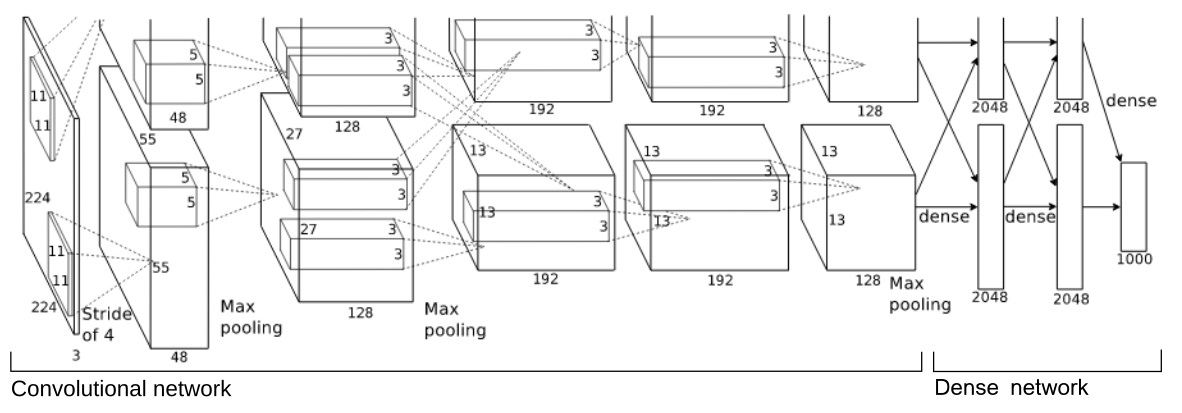
\includegraphics[width=\linewidth]{imagenet-arch}}
\end{figure}

Como explicamos en la sección \ref{sec:conv-net}, cuando una red convolucional
recibe una imagen devuelve $N$ matrices bidimensionales representando el
resultado de la aplicación de los $N$ conjuntos de filtros a la imagen inicial.
Intuitivamente podemos pensar que la salida de cada uno de estos filtros
representa la aparición en la imagen de la característica que esté detectando
el filtro. Necesitamos entonces que en las últimas capas la red aprenda
filtros que se activen sólo con la aparición de una clase de pez.

Un detalle que debemos tener en cuenta que este modelo convolucional no ha sido entrenado con el conjunto de entrenamiento del problema, sino con el conjunto de entrenamiento de \cite{imagenet}. Por lo tanto, nuestro uso de esta red convolucional será únicamente para transformar cada imagen del conjunto de entrenamiento del problema a un conjunto de características.

La arquitectura del artículo original \parencite{krizhevsky2012imagenet} usa
capas convolucionales donde alterna filtros de $11\times11$, $5\times5$ y
$3\times3$, el cual parece una buena elección para usar como modelo
convolucional preentrenado. Sin embargo, la aplicación de este trabajo es una
competición internacional donde se usarán soluciones \textit{state of the art}.
El modelo de la figura \ref{general-architecture} representa el ganador de la
edición 2012 de la competición ILSVRC, hace ya cinco años, por lo que resulta
conveniente analizar cuales fueron los ganadores de años posteriores.

El modelo principal que usaremos es VGG, desarrollado por el \textit{Visual
Geometry Group}, de la Universidad de Oxford \parencite{simonyan}. Es un modelo
especialmente interesante por su simplicidad, aparte de obtener una de las
mejores puntuaciones en ILSVRC 2014. Una de las principales características de
VGG es la idea de que los filtros convolucionales mayores de $3\times3$, como
por ejemplo los de $5\times5$ u $11\times11$, pueden ser representados por
combinaciones de filtros $3\times3$.

De las configuraciones descritas en \parencite{simonyan} hay una que sobresale
por su eficiencia, llamada VGG16. Usando un total de trece capas CONV con
filtros de $3\times3$, cinco capas POOL y tres capas FC (de 4096, 4096 y 1000
salidas), seguida de una función \textit{softmax} (figura \ref{vgg16-arch}), es
capaz de mejorar la eficacia del modelo de Krizhevsky. El nombre de esta
configuración es VGG16, por ser esta la cantidad de capas CONV y FC que posee.

\begin{figure}
  \caption{Arquitectura de VGG}
\label{vgg16-arch}
  \makebox[\textwidth]{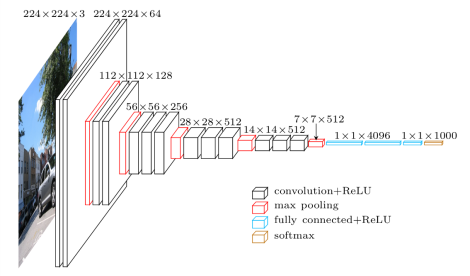
\includegraphics[width=.7\linewidth]{vgg16-arch}}
\end{figure}

\subsection{Ajuste fino}

Si observamos la última capa del modelo VGG16, vemos que la salida tiene 1000
elementos. Tiene esta forma ya que ILSVRC consiste en clasificar una imagen
entre mil categorías diferentes. Como en nuestro problema solo tenemos ocho
categorías, es lógico modificar esta última capa para que únicamente tenga ocho
salidas.

Al modificar la estructura de la última capa estamos destruyendo pesos y
haciendo que muchos de los que ya existían carezcan de sentido. El hecho de que
VGG una esta separación lógica entre la red convolucional y la red densa hace
que se pueda separar el modelo en dos submodelos diferentes: uno convolucional,
que no habrá cambiado con la adaptación a las ocho categorías, y otro denso,
que tendrá que ser entrenado de nuevo.

Esta técnica de ajustar los parámetros de un modelo ya conocido para adaptarlo
a un nuevo conjunto de datos se conoce como ajuste fino (\textit{fine-tuning}).
En la figura \ref{basic_architecture} se puede ver un resumen de las diferentes
etapas por los que pasa la red.

Al dividir la red en dos subredes diferentes hay que tener en cuenta que la
segunda, la red densa, no recibe como entrada las imágenes, sino la salida de
la primera red convolucional, con todas las transformaciones que esta produce.
Es necesario entonces aplicar la red convolucional a nuestro conjunto de datos
de entrenamiento para crear un nuevo conjunto de datos con el que reentrenar la
red densa.

\begin{figure}
  \caption{Estructura del modelo final. Como recibe como entrada imágenes de 244 píxeles, pasa por las diferentes redes y devuelve el vector de ocho categorías.}
\label{basic_architecture}
  \makebox[\textwidth]{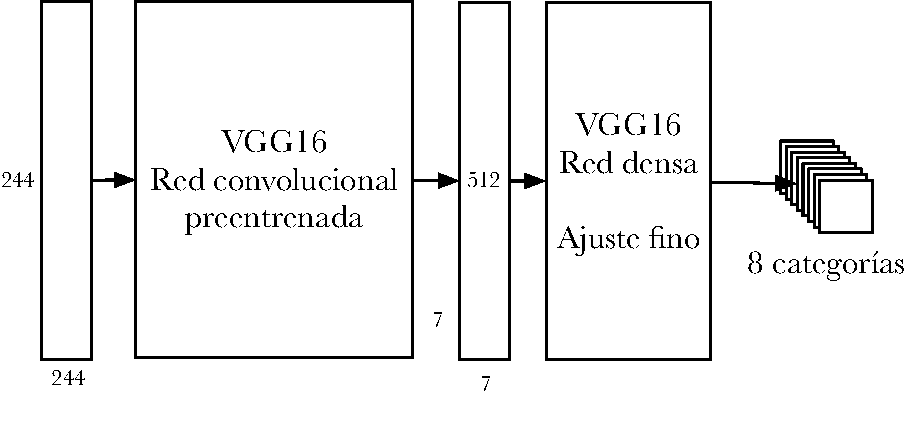
\includegraphics[width=.7\linewidth]{basic_architecture}}
\end{figure}

El siguiente código (simplificado) realiza esta tarea para los subconjuntos
locales de entrenamiento, validación y prueba.

\begin{python}
# Carga del modelo VGG16
from vgg16 import Vgg16
model = Vgg16()

# Separacion entre red convolucional y densa
import utils
conv_model, dense_model = utils.split_at(model, MaxPooling2D)

# Carga de los diferentes conjuntos de datos
#  'path' es la carpeta donde se encuentra los
#  conjuntos de datos
train, train_labels = get_data(path + 'train')
valid, valid_labels = get_data(path + 'valid')
test, test_labels = get_data(path + 'test')

# Conversion a caracteristicas mediante la red convolucional
train_feat = conv_model.predict(train)
valid_feat = conv_model.predict(valid)
test_feat = conv_model.predict(test)

# Sustitucion de la capa de salida
dense_model.pop()  # Eliminar la capa final
dense_model.add(
    Dense(8, activation='softmax')  # Introducir una nueva capa
)

# Compilacion del modelo
dense_model.compile(
    SGD(lr=0.01),  # Factor de aprendizaje
    loss='categorical_crossentropy',
    metrics=['accuracy'],  # Muestra la precision del modelo
)

# Entrenamiento de la red
dense_model.fit(
    train_feat,
    train_labels,
    batch_size=64,  # Numero de imagenes a entrenar al mismo tiempo
    nb_epoch=7,     # Numero de iteraciones del entrenamiento
    validation_data=(valid_feat, valid_labels),
)

# Evaluar el modelo sobre el conjunto de test
dense_model.evaluate(test_feat, test_labels)
# Log loss, accuracy
>>> [1.90571456890184755, 0.66099843993759748]
\end{python}

La puntuación total para el conjunto de test local sería 1.906. 

El segundo número que devuelve la función $evaluate$ es la precisión
($accuracy$) del modelo. Al ser este un modelo de clasificación, la precisión
es el porcentaje de veces que la clase con la probabilidad máxima se
corresponde con la clase etiquetada en el conjunto de datos. En este caso la
red ha clasificado correctamente el 66 \% de las imágenes, un número muy
aceptable teniendo en cuenta que solo se ha tocado la capa final de un modelo
ajeno.

Al subir a \textit{Kaggle} las predicciones del modelo sobre el conjunto de
prueba de la primera fase de la competición se obtuvo una puntuación de pérdida
logarítimica de \textbf{2.632}. Aunque el error ha aumentado sensiblemente esto es
perfectamente normal, ya que las imágenes proporcionadas al modelo son
completamente nuevas. Lo interesante será comparar esta puntuación con las de otros modelos sobre el mismo conjunto de test.

\section{Modelo completamente conectado}
\label{sec:model_connected}

El modelo original de VGG usa dos capas $densas$ de 4096 neuronas para
clasificar entre mil clases diferentes. Ya que nuestro problema tiene solo ocho
clases diferentes probablemente no sea necesario usar capas tan grandes, por lo
que se procede a probar la misma estructura original, pero con capas cuatro
veces más pequeñas que las originales.

La estructura, por lo tanto, quedaría de la misma manera pero usando dos capas
densas de 512 neuronas cada una y una capa densa final de 8 (figura
\ref{standard_arch}). En vez de separar la parte convolucional de la densa en el modelo y modificar la densa cada vez que haya que probar una idea diferente, es más sencillo crear una red neuronal nueva con $Keras$, y añadir todas las capas necesarias.

\begin{figure}
  \caption{Arquitectura del modelo completamente conectado}
\label{standard_arch}
  \makebox[\textwidth]{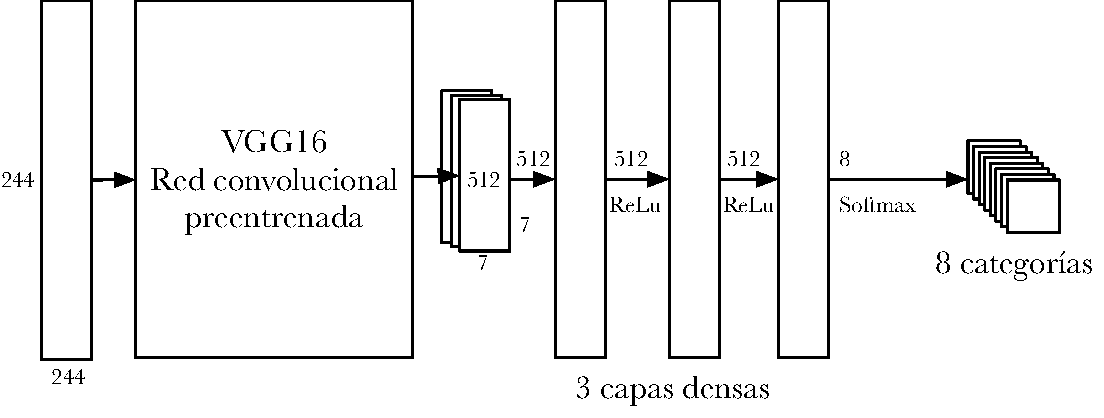
\includegraphics[width=.9\linewidth]{standard_arch}}
\end{figure}

Un paso importante a la hora de construir el modelo personalizado es tener en cuenta que las salidas de las redes convolucionales poseen tres dimensiones ($ancho \times alto \times filtros$), mientras que la redes neuronales densas poseen solo una dimensión. Es necesario convertir la salida de estas capas a una entrada permitida. \textit{Keras} ya ofrece esta posibilidad usando una capa abstracta llamada \textit{Flatten}.

\begin{python}
def list_dense_layers():
    return [
        Flatten(),
        Dense(512, activation='relu'),
        Dense(512, activation='relu'),
        Dense(8, activation='softmax')
    ]

dense_model = keras.models.Sequential(list_dense_layers())

# Entrenar la red
dense_model.compile(...)
dense_model.fit(...)

# Evaluar el modelo sobre el conjunto de test
dense_model.evaluate(test_feat, test_labels)
>>> [1.27161316430079874, 0.73067862714508579]
\end{python}

Los resultados obtenidos son ligeramente mejores que los anteriores. Sin
embargo no es aquí donde está toda la mejora. El entrenamiento de este modelo
ha sido un 80\% más rápido que el anterior (19.5 segundos por iteración en el
primero, 3.9 segundos en este último). Esto no solo ha permitido entrenar la
red durante más tiempo, sino que en el futuro hará posible entrenar sobre
mayores cantidades de datos sin aumentar excesivamente el tiempo de entrenamiento.

La puntuación en la tabla pública de \textit{Kaggle} para este modelo ha sido
de \textbf{2.381}.

\subsection{Análisis del sobreajuste}

La salida de \textit{Keras} al entrenar el modelo ofrece información de lo que
está sucediendo. Este es un ejemplo de la salida del entrenamiento del modelo
anterior.

\begin{python}
Epoch 5/7
loss: 0.354 - acc: 0.992 - val_loss: 1.091 - val_acc: 0.872
Epoch 6/7
loss: 0.253 - acc: 0.996 - val_loss: 0.995- val_acc: 0.881
Epoch 7/7
loss: 0.193 - acc: 0.997 - val_loss: 0.987- val_acc: 0.913
\end{python}

En cada una de las iteraciones del entrenamiento, \textit{Keras} muestra los
valores de aplicar el modelo actual a los ejemplos de entrenamiento y
validación. Se puede observar que el modelo funciona mucho mejor en el conjunto
de entrenamiento que en el de validación.

Cuando un modelo tiene demasiados parámetros y ha sido entrenado durante demasiado tiempo aprende a clasificar los ejemplos con los que entrena usando información específica de cada uno de ellos en vez de generalizar. Esto se conoce como \textbf{sobreajuste} (\textit{overfitting}).

Los datos del modelo anterior indican que puede existir un sobreajuste, por lo que se va a intentar tomar medidas para arreglarlo.

\subsection{\textit{Dropout}}
\label{sec:dropout}

Una de las características de VGG y otras redes convolucionales es el uso de
\textit{dropout} para reducir el sobreajuste de los modelos entrenados. El
\textit{dropout} consiste en una capa que se aplica después de las capas de
activación de las capas densas. Esta capa convierte activaciones aleatorias a
0, eliminando la información transportada (Figura \ref{dropout-net})

\begin{figure}
    \caption{A la izquierda una red neuronal estándar con dos capas ocultas. A la derecha la misma red aplicando un \textit{dropout} en cada una de las capas ocultas. Las neuronas tachadas han perdido su activación.}
\label{dropout-net}
  \makebox[\textwidth]{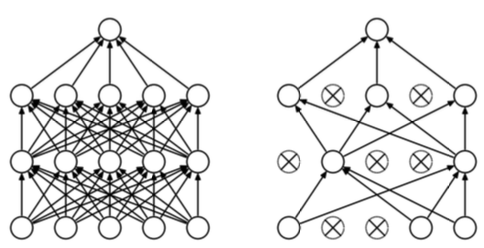
\includegraphics[width=0.7\linewidth]{dropout-net}}
\end{figure}

En un principio parecería que esto perjudica al modelo, pero al eliminar algunos de los pesos el modelo evita centrarse en características individuales de cada ejemplo de clasificación, obligándolo a generalizar más rápido \parencite{dropout}.

Un pequeño experimento en un modelo más avanzado (VGG con normalización por lotes y aumento de datos) permite ver cómo afecta el \textit{dropout} a la puntuación final. En la figura \ref{dropout} se puede observar que la mejor puntuación se alcanza eliminando el 45 \% de las activaciones, consiguiendo una mejora de un 25 \% sobre el modelo que usa todas las activaciones.

\begin{figure}
    \caption{Evolución de la puntuación de un modelo usando \textit{dropout}}
\label{dropout}
  \makebox[\textwidth]{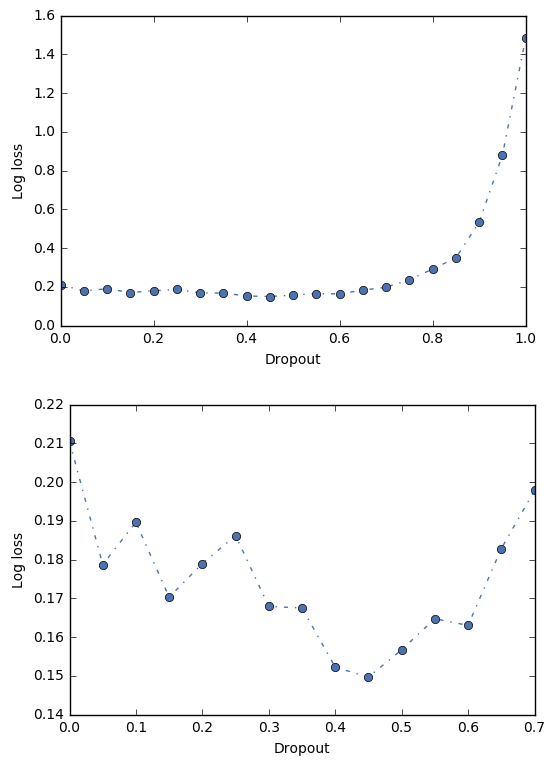
\includegraphics[width=0.7\linewidth]{dropout}}
\end{figure}

También se ve que el modelo empieza a perder eficacia a partir del 70 \% de \textit{dropout}, empeorando el modelo original. Esto significa que el modelo es capaz de generalizar con información útil incluso cuando solo posee el 30 \% de las activaciones.

Por otra parte, también es importante pensar dónde se pierden las activaciones.
Por un lado, perder demasiadas activaciones en la entrada sería el equivalente
a trabajar sin esos ejemplos. Por otro, perderlos en la salida sería aumentar
demasiado el error al clasificar, al no tener tanta capacidad de apoyo en las
otras capas.  La idea aplicada aquí es distribuir el \textit{dropout}
disminuyéndolo en la entrada y la salida y haciendo que alcance máximo
en el centro de la red.

El modelo modificado quedaría de la siguiente manera:

\begin{python}
def list_dense_layers(dropout):
    return [
        Flatten(),
        Dropout(dropout/4),  # Aplicar 1/4 del dropout definido 
        Dense(512, activation='relu'),
        Dropout(dropout),
        Dense(512, activation='relu'),
        Dropout(dropout/2),  # Aplicar la mitad del dropout definido
        Dense(8, activation='softmax'),
    ]
dense_model = keras.models.Sequential(list_dense_layers(0.45))
\end{python}

Los resultados obtenidos con esta configuracion no mejoran los resultados de la red anterior, pero como se ve en la figura \ref{dropout} sí que lo hará a posteriori, cuando se le apliquen otro tipo de modificaciones al modelo. Modelos como VGG ya incluyen \textit{dropout} (solo en las redes densas), por lo que al hacer fine-tuning con una red personalizada es necesario usarlo para mantener los resultados originales.

\subsection{Normalización por lotes}

En muchos campos del aprendizaje automático es habitual normalizar las entradas
de los modelos. Si existe una entrada mucho mayor o menor que el resto esta
puede hacer que el entrenamiento arrastre un error mayor del necesario,
produciendo inestabilidad y dificultando la convergencia del modelo. Normalizar
un conjunto de entradas hace que todas estén en la misma escala. 

El caso de las redes neuronales no es una excepción. Una entrada con un valor
demasiado grande puede llevar a tener un peso determinado demasiado grande para
contrarrestarla.

Una normalización estándar en aprendizaje automático es restar de cada entrada
el valor medio del conjunto de datos y luego dividirlo por la desviación
estándar del mismo. Esto aún presenta problemas para casos como el de este
proyecto donde se usan algoritmos como el gradiente del descenso estocástico
para la propagación hacia atrás (sección \ref{sec:backprop}).

Los modelos principales citados en este trabajo,
\parencite{krizhevsky2012imagenet} y \parencite{simonyan}, usan sus propias
técnicas de normalización, aparte de usar activaciones \textit{ReLu} (sección
\ref{sec:relu}) que son menos sensibles a los datos de entrada sin normalizar.
Sin embargo, en 2015 se presenta una técnica muy interesante de normalización
que cuadra muy bien con el gradiente del descenso estocástico: la normalización
por lotes (\textit{batch normalization}) \parencite{batch_normalization}.

La diferencia con una normalización estándar es que tras normalizar las
entradas de una capa se multiplican por un parámetro aleatorio y luego se
suma otro, cambiando así la desviación estándar y la media de la entrada. Estos
dos parámetros se hacen entonces entrenables como pesos del modelo.

Los modelos actuales que usan esta normalización por lotes consiguen la misma
precisión que los modelos sin ella usando catorce veces menos pasos de
entrenamiento \parencite{batch_normalization}.

Para aplicar esta normalización por lotes al modelo que se está entrenando hay
que añadir las capas de normalización por lotes (también disponibles en
\textit{Keras}) al modelo denso:

\begin{python}
def list_dense_layers(dropout):
    return [
        BatchNormalization(axis=1),
        Flatten(),
        Dropout(dropout/4),
        Dense(512, activation='relu'),
        BatchNormalization(),
        Dropout(dropout),
        Dense(512, activation='relu'),
        BatchNormalization(),
        Dropout(dropout/2),
        Dense(8, activation='softmax'),
    ]
dense_model = keras.models.Sequential(list_dense_layers(0.45))
\end{python}

Esto no es suficiente. A diferencia del \textit{dropout}, la normalización por
lotes sí que es capaz de mejorar la red convolucional del modelo preentrenado.
Gracias a la popularidad de esta técnica y de los modelos preentrenados que se
usan en este trabajo, ya existen entrenamientos del modelo VGG original usando
normalización por lotes, ahorrando la necesidad de entrenar una red tan grande.
Una descripción de estos entrenamientos se puede encontrar en
\parencite{pretrained_with_bn}.

En el caso de este trabajo se ha adaptado la clase $Vgg16BN$, siguiendo
los principios descritos en \parencite{fastai}. Al cambiar la red convolucional
original hay que volver a transformar el conjunto de datos que se usaba para
obtener los resultados de aplicar los filtros actualizados sobre las imágenes
de entrada.

\begin{python}
# Carga del modelo VGG16 con normalizacion por lotes
from vgg16bn import Vgg16BN
import utils
model = Vgg16BN()
conv_model, _ = utils.split_at(model, MaxPooling2D)

# Carga de los diferentes conjuntos de datos
train, train_labels = get_data(path + 'train')
valid, valid_labels = get_data(path + 'valid')
test, test_labels = get_data(path + 'test')

# Conversion a caracteristicas mediante la red convolucional
train_feat = conv_model.predict(train)
valid_feat = conv_model.predict(valid)
test_feat = conv_model.predict(test)

# Entrenamiento la red
dense_model = keras.models.Sequential(list_dense_layers(0.45))
dense_model.compile(...)
dense_model.fit(...)
# Evaluacion del modelo sobre el conjunto de test
dense_model.evaluate(test_feat, test_labels)
>>> [0.45127591543710, 0.96109451984491]
\end{python}

Como se puede apreciar, los dos últimos cambios han supuesto una mejora considerable sobre el modelo anterior, clasificando correctamente el 96\% de los ejemplos del conjunto de test.

La puntuación en la tabla pública de \textit{Kaggle} para este modelo ha sido
de \textbf{1.017}.


\subsection{Aumento de datos}

Uno de los principales obstáculos de este problema es el reducido tamaño del conjunto de datos de entrenamiento. El tener pocos ejemplos sobre los que entrenar hace que al modelo le cueste generalizar sobre los ejemplos disponibles, produciéndose un sobreajuste.

Para tratar de reducir el sobreajuste del modelo se puede usar una técnica
llamada aumento de datos (\textit{data augmentation}). Consiste en generar
imágenes de entrenamiento adicionales a partir de las ya disponibles, rotando
la imagen original, aumentándola, cambiando ligeramente el color, etc.

En el caso de nuestro problema esta técnica es especialmente interesante, ya
que las cámaras de los barcos están fijas apuntando siempre a la misma zona. En
las fotos sobre los peces capturados estos siempre suelen estar con la cabeza
apuntando en dirección contraria al agua. Ello hace que la red reconozca más
fácilmente peces dispuestos en una determinada dirección, costándole más
trabajo para el resto de direcciones. Si las redes convolucionales ayudaban a
detectar determinados patrones en cualquier punto de la imagen, el aumento de
datos hace lo propio de otras variantes como la rotación, el tamaño o el filtro
de color dado por el ambiente.

Un ejemplo de aumento de datos se muestra en la figura \ref{augmentations}, que contiene cuatro imágenes obtenidas al reescalar de distintas maneras la imagen original de la figura \ref{aug-original}.

\begin{figure}
    \caption{Imagen del conjunto de datos}
\label{aug-original}
  \makebox[\textwidth]{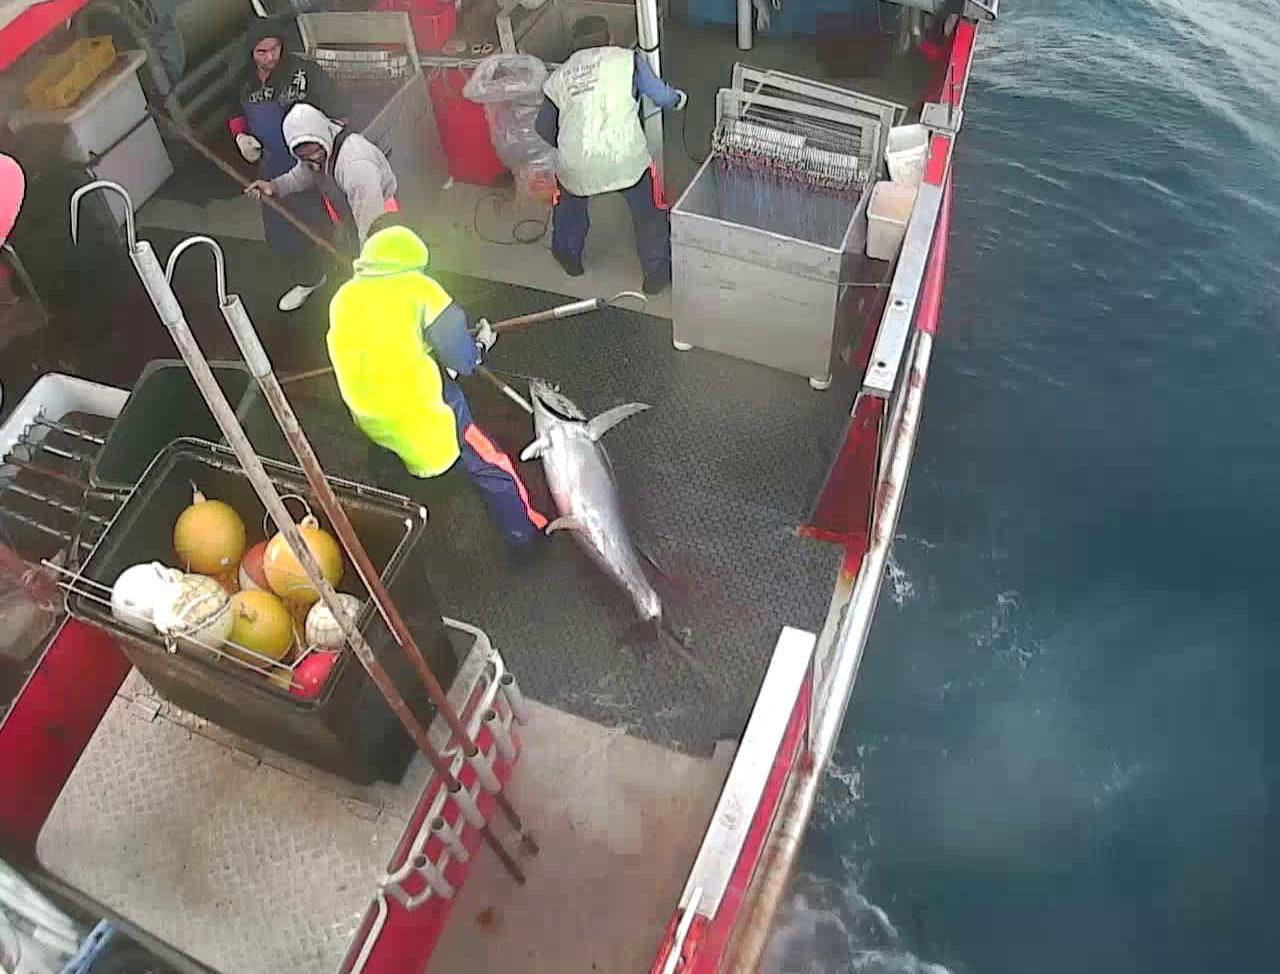
\includegraphics[width=0.7\linewidth]{aug-original}}
\end{figure}

\begin{figure}
    \caption{Cuatro aumentos diferentes de la imagen, reescalada a $224\times224$ píxeles}
\label{augmentations}
  \makebox[\textwidth]{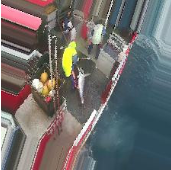
\includegraphics[width=.2\linewidth]{au1}}
  \makebox[\textwidth]{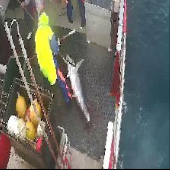
\includegraphics[width=.2\linewidth]{au3}}
  \makebox[\textwidth]{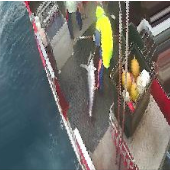
\includegraphics[width=.2\linewidth]{au2}}
  \makebox[\textwidth]{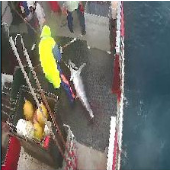
\includegraphics[width=.2\linewidth]{au4}}
\end{figure}

Para trabajar con aumentos de datos, \textit{Keras} proporciona una serie de
opciones de transformación dentro de la utilidad para importar conjuntos de
datos. Al definir dichas opciones, como por ejemplo rotación, zoom o volteo
horizontal, \textit{Keras} generará nuevas imágenes a la vez que carga el
conjunto de datos en memoria.

Si es necesario conocer cómo se aplican las transformaciones a las diferentes imágenes, es posible especificar un directorio de salida del generador de imágenes, de tal manera que los resultados de las distintas transformaciones se guarden en directorios particulares.

\begin{python}
# Creacion del generador de imagenes
image_generator = image.ImageDataGenerator(
    rotation_range=30,
    horizontal_flip=True,
    zoom_range=0.4,
)

batches = img_generator.flow_from_directory(
    path+'test_aug',
    target_size=(224,224),
    class_mode='categorical',
    shuffle=False,
    batch_size=4,
    save_to_dir=path+'augmentation',
)

# Iteracion sobre lotes para extraer los datos
# En este caso se sacan 4 veces la cantidad de datos originales
data = [batch.next() for _ in range(batches.nb_samples * 4)]
\end{python}

Ahora no es necesario modificar el modelo, solo reentrenarlo con los nuevos datos. Como ha ocurrido antes, al cambiar el conjunto de datos hay que transformarlo pasándolo por la red convolucional, usando en este caso la última versión con normalización por lotes.

Lo interesante en este caso es la reducción del sobreajuste que se ha obtenido.

\begin{python}
Epoch 5/7
loss: 0.0768 - acc: 0.9817 - val_loss: 0.1142 - val_acc: 0.9538
Epoch 6/7
loss: 0.0639 - acc: 0.9895 - val_loss: 0.1212 - val_acc: 0.9334
Epoch 7/7
loss: 0.0708 - acc: 0.9860 - val_loss: 0.1139 - val_acc: 0.9520

dense_model.evaluate(test_feat, test_labels)
>>> [0.31255581648, 0.96723868954]
\end{python}

El modelo, que ahora ha predicho correctamente casi un 97\% de las imágenes del conjunto de test, ha disminuido ligeramente la puntuación de pérdida logarítmica. Hay que tener en cuenta que a medida que esta puntuación tiende a cero, es más difícil disminuirla, ya que corresponde cada vez más a un modelo casi perfecto.

Cuando hablamos de un modelo casi perfecto, nos referimos respecto al conjunto de test elegido. En este caso, debido al pequeño tamaño del conjunto de test, la perfección del modelo estará lejos de la perfección del modelo real que va a ser probado en el reto.

La puntuación en la tabla pública de \textit{Kaggle} para este modelo ha sido
de \textbf{0.9364}, el mejor hasta ahora.

\section{Modelo convolucional}

Hasta ahora se ha seguido siempre el mismo esquema: una vez transformado el
conjunto de datos entrenamos una red densa (completamente conectada) de tres
capas. Además, una parte del preprocesamiento de las imágenes consiste en
redimensionarlas a un tamaño más manejable, de $224\times224$ píxeles.

Una de las ventajas de las redes convolucionales es que permite aumentar el
tamaño de las imágenes elegidas sin que por ello se incremente la complejidad
de la red, ya que el número de pesos no cambiaría, solo el tamaño de la salida.
Sin embargo, la complejidad de la red neuronal estándar que hemos colocado tras
la red convolucional sí que vería incrementarse muchísimo su complejidad con el
cambio de tamaño de las imágenes.

Para intentar aprovechar esta ventaja que ofrecen las redes convolucionales
frente a las redes densas, se puede intentar trabajar usando solo capas
convolucionales en todo el proceso, clasificando al final con una única capa de
activación clásica.

Aquí se estaría desarrollando una idea que se comentaba al principio de este
trabajo, el conseguir ocho filtros cuya salida sea la probabilidad de que en la
zona de la imagen esté apareciendo el pez de la clase elegida.

Se usarán inicialmente tres capas de convoluciones, con 128 filtros cada una.
La combinación de estos 128 filtros permitirá capturar la combinatoria de
caracterísicas que representa la red convolucional preentrenada. Al final se
añade una última capa de convolución con 8 filtros, el mismo número de
categorías en las que clasificar.

Las imágenes resultantes de estos filtros se transforman a una sola salida
mediante una capa \textit{GlobalAveragePooling2D}. Esta capa funciona como las
capas POOL de la red convolucional, pero usando la media del total de los
píxeles de la imagen, generando una salida de un valor por filtro que pueda ser
entendida por la capa de activación.

La arquitectura final de la red se muestra en la figura \ref{fcn_arch}.

\begin{python}
def build_conv_layers():
    return [
        BatchNormalization(axis=1,
            input_shape=conv_layers[-1].output_shape[1:]
        ),
        Convolution2D(128, 3, 3, activation='relu', border_mode='same'),
        BatchNormalization(axis=1),
        Convolution2D(128, 3, 3, activation='relu', border_mode='same'),
        BatchNormalization(axis=1),
        Convolution2D(128, 3, 3, activation='relu', border_mode='same'),
        BatchNormalization(axis=1),
        Convolution2D(8, 3, 3, border_mode='same'),

        # Output layer
        GlobalAveragePooling2D(),
        Activation('softmax'),
    ]
\end{python}


\begin{figure}
    \caption{Arquitectura de la red completamente convolucional}
\label{fcn_arch}
  \makebox[\textwidth]{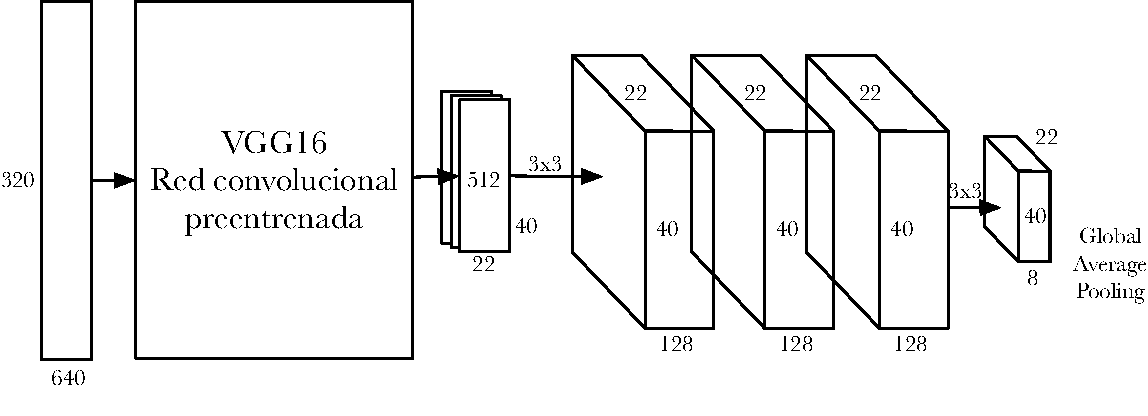
\includegraphics[width=0.7\linewidth]{fcn_arch}}
\end{figure}

De nuevo habrá que transformar el conjunto de datos por medio de la red
convolucional preentrenada, ya que se va a usar un tamaño de imagen de
$360\times640$. Aunque, como se ha comentado, la red convolucional admite un
aumento del tamaño de la imagen sin que crezca exponencialmente el tiempo de
entrenamiento, el entrenamiento de una red convolucional es mucho más costoso
que el de una red clásica. Esto se debe a que hay que actualizar $n\timesn$
pesos por cada píxel de cada imagen. En este caso el entrenamiento de la red
completamente convolucional ha tardado 24 veces más que el entrenamiento de la
red densa del capítulo anterior.

\begin{python}
conv_model.evaluate(test_feat, test_labels)
>>> [0.243715549991, 0.969645081488]
\end{python}

Al evaluar el modelo se ve que consigue una pequeña mejora respecto al modelo
denso. La puntuación en la tabla pública de \textit{Kaggle} para este modelo ha
sido de \textbf{0.8109}.


\subsection{Visualización del modelo}

El trabajar en todo momento (salvo en la última capa) con redes
convolucionales, implica que los pesos son siempre filtros que se aplican a
imágenes. Se pretende entonces conseguir filtros que resalten la existencia en
cada zona de la imagen de un pez de una determinada clase.

Se pueden usar los diferentes valores de los filtros para construir un mapa de
calor para la categoría que le corresponde. Un mapa de calor es una
representación gráfica de los valores de una matriz bidimensional. Generalmente
valores pequeños se asocian a colores más claros, como el azul o el verde, y
valores mayores a colores más cálidos, como el rojo o el morado.

Si se redimensiona el filtro (ya que ha sido reducido por las capas de
\textit{MaxPooling2D}) al tamaño de la imagen original, se puede ver cómo
encuentra el pez a clasificar en cada imagen. Como ejemplo, al aplicar la red a
la imagen de la figura \ref{fc-fish} podemos visualizar el filtro perteneciente
a su categoría (ALB: \textit{Thunnus alalunga}) en la figura \ref{fc-heatmap}.

\begin{figure}
    \caption{Una imagen correspondiente a la clase ALB: \textit{Thunnus alalunga}}
\label{fc-fish}
  \makebox[\textwidth]{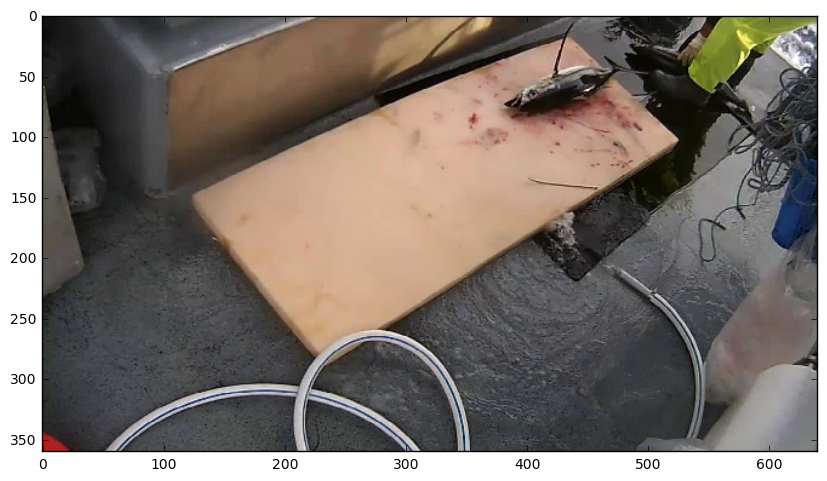
\includegraphics[width=\linewidth]{fc-fish}}
\end{figure}

\begin{figure}
    \caption{Aplicación del mapa de calor reescalado a la imagen de la figura \ref{fc-fish}}
\label{fc-heatmap}
  \makebox[\textwidth]{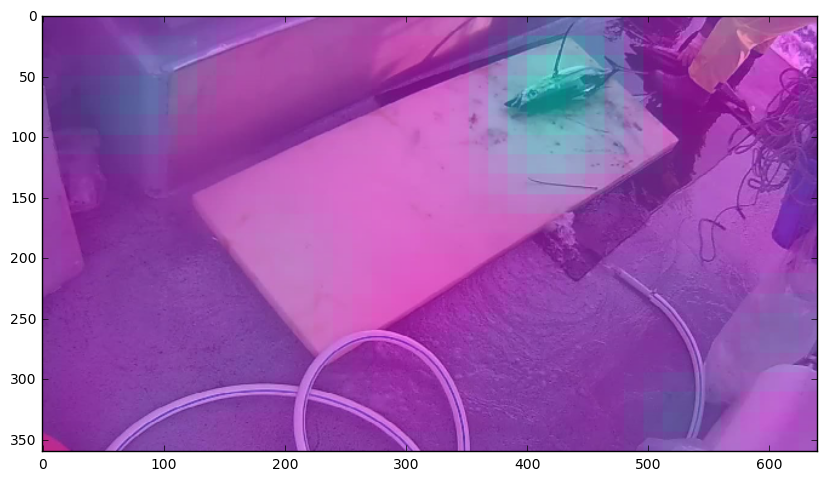
\includegraphics[width=\linewidth]{fc-heatmap}}
\end{figure}

Esto no solo permite comprobar que el modelo funciona correctamente, sino también buscar los ejemplos que peor clasifica y analizar qué está señalando el mapa de calor correspondiente.

Un ejemplo claro de cómo se puede usar esta técnica de visualización para
detectar los errores en el modelo es el intento de clasificación un atún de
cola amarilla (YFT: \textit{Thunnus albacares}), en la imagen de la figura
\ref{yft}. Una característica de los atunes de cola amarilla es su banda de
tonos amarillos en el lomo, característica que el modelo podría haber aprendido
gracias a los ejemplos. Sin embargo, la imagen muestra el atún visto
desde abajo, con las aletas abiertas. Esto esconde una de las principales
características del atún, siendo difícil clasificarlo incluso para un humano no
familiarizado con atunes.

Al mostrar el mapa de calor correspondiente (figura \ref{yft-heatmap}) se puede
apreciar que la hipótesis de que el modelo ha aprendido a detectar los atunes
de cola amarilla a través del color podría ser cierta, ya que una de las partes
más importantes de la foto para el filtro son los pantalones del pescador, de
un color amarillo fuerte.

Esto permite tomar ciertas decisiones sobre el entrenamiento del modelo. Por
ejemplo, si se ve que la fijación del modelo con el color es un error y es
preferible que use otras cosas como formas o texturas, se puede eliminar el
color de las imágenes o aumentar los datos usando transformaciones de color que
hagan especial hincapié en la varianza del color amarillo.

\begin{figure}
    \caption{Una imagen correspondiente a la clase ALB: \textit{Thunnus alalunga}}
\label{yft}
  \makebox[\textwidth]{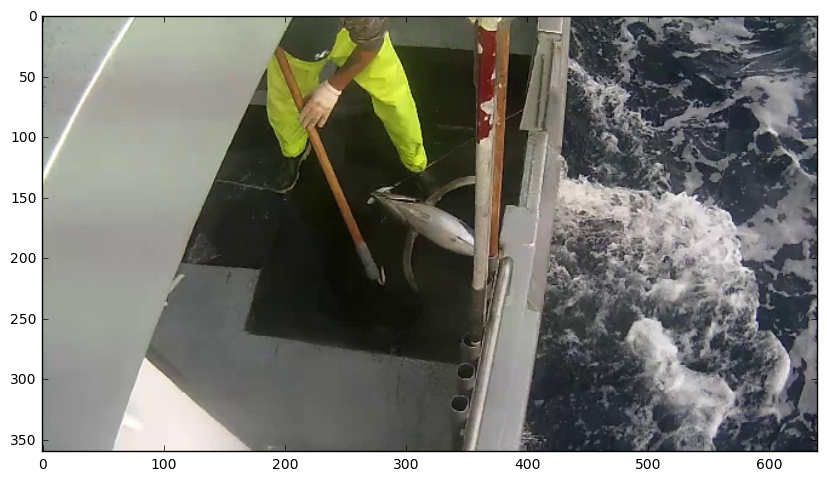
\includegraphics[width=\linewidth]{yft}}
\end{figure}

\begin{figure}
    \caption{Aplicación del mapa de calor reescalado a la imagen \ref{fc-fish}}
\label{yft-heatmap}
  \makebox[\textwidth]{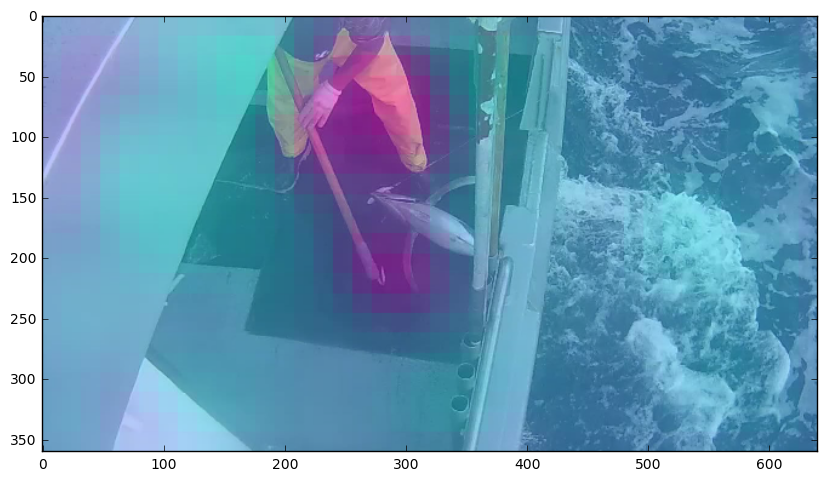
\includegraphics[width=\linewidth]{yft-heatmap}}
\end{figure}

\section{Modelo con entrada múltiple}
\label{sec:multi_entry}

Como se vió en el análisis del conjunto de datos (sección \ref{dataset}), hay
otras propiedades de las imágenes cuyo uso podría permitir una mejora de los
modelos. Por ejemplo, las imágenes están tomadas en diferentes barcos, con
diferentes modelos de cámaras. No todas las cámaras generan imágenes del mismo
tamaño, por lo que se podría averiguar el barco del que se ha tomado la
fotografía por el tamaño de la imagen.

Ya que cada barco suele pescar diferentes tipos de peces con mayor o menor
probabilidad, el conocer el tipo de barco puede ser aprovechado por el modelo
para balancear las posibilidades de cada categoría dependiendo del tipo de
pesca que suela llevar.

La idea no es hacer todo esto a mano, sino entrenar un modelo que tenga en
cuenta tanto las imágenes como otra información válida; en este caso, cual es
el tamaño de la imagen. En el conjunto de datos hay diez tamaños diferentes de
imágenes, las cuales se codificarán en \textit{onehot} para facilitar el
entrenamiento.  Los diferentes tamaños de las imágenes son los indicados en el
cuadro \ref{image_sizes}.

\begin{table}[]
\centering
\caption{Ocurrencia de los diferentes tamaños de imagen}
\label{image_sizes}
\begin{tabular}{rr}
\textbf{Tamaño de la imagen} & \textbf{Cantidad de imágenes} \\
1192 \times 670              & 169                           \\
1276 \times 718              & 192                        \\
1244 \times 700              & 23                            \\
1280 \times 720              & 1880                          \\
1280 \times 750              & 520                           \\
1280 \times 924              & 51                            \\
1280 \times 974              & 344                           \\
1334 \times 750              & 28                            \\
1518 \times 854              & 37                            \\
1732 \times 974              & 33                           
\end{tabular}
\end{table}

Para la arquitectura del modelo vamos a usar la red densa, con la diferencia de
que la última capa tendrá dos entradas: la salida de las capas ocultas de la
red neuronal y la clasificación del tamaño de la imagen, codificado en
\textit{onehot}, como se muestra en la figura \ref{multi_input_arch}.

\begin{figure}
    \caption{Arquitectura del modelo con entrada múltiple}
\label{multi_input_arch}
  \makebox[\textwidth]{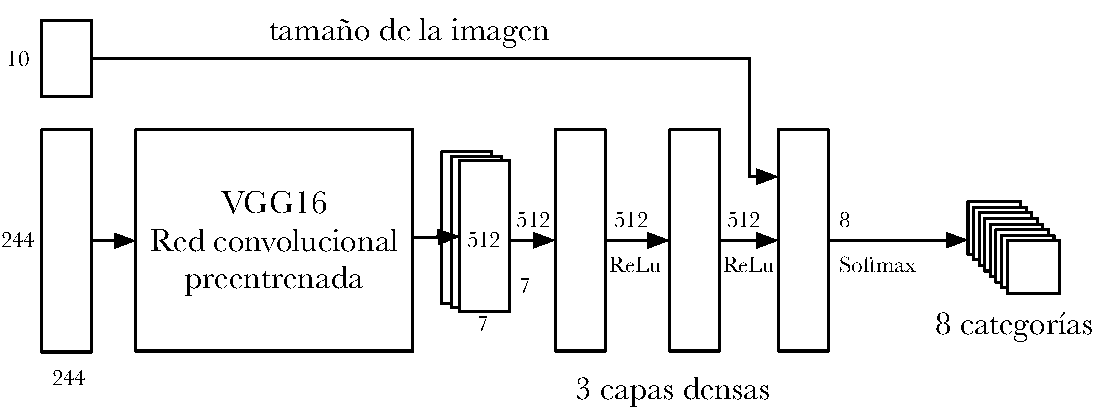
\includegraphics[width=\linewidth]{multi_input_arch}}
\end{figure}

La estructura del código es ligeramente diferente, ya que ahora vamos a generar
todas las capas que teníamos anteriormente menos la última en una misma
función:

\begin{python}
def build_dense_layers(dropout=0.5):
    # Usamos las entradas de la red convolucional, como antes
    inp = Input(conv_layers[-1].output_shape[1:])
    x = MaxPooling2D()(inp)
    x = BatchNormalization(axis=1)
    x = Flatten()
    x = Dropout(dropout/4)
    x = Dense(512, activation='relu')
    x = BatchNormalization()
    x = Dropout(dropout)
    x = Dense(512, activation='relu')
    x = BatchNormalization()
    x = Dropout(dropout/2)
    return x

\end{python}

Usando esta función, añadimos una capa final para la clasificación, cuya entrada
será la union entre la red densa y la información sobre los tamaños de las
imágenes. Esta capa deberá clasificar cada imagen usando tanto la información
disponible de la red densa como el barco al que pertenece.

\begin{python}
# Generar las capas de la red
net = build_dense_layers()

# Usar las entradas de las dimensiones de cada elemento
size_inputs = Input(len(sizes))
bn_inputs = BatchNormalization()(size_inputs)

# Unir las dos entradas en una sola capa
net = merge([net, bn_inputs], 'concat']
net = Dense(8, activation='softmax')(net)

# Crear la red
dense_model = keras.models.Model(
    [inp, size_inputs],  # El modelo ahora tiene multientrada
    net
)
\end{python}

Tras construir el modelo con las entradas múltiples y entrenarlo sobre los dos
conjuntos de entrenamiento (las imágenes y los tamaños de las imágenes) vemos
la evaluación del modelo.

\begin{python}
dense_model.evaluate(test_feat, test_labels)
>>> [0.373333961543, 0.941351055711]
\end{python}

El modelo ha sacado una evaluación peor que modelos anteriores, incluso usando
un modelo que ya se conocía con una evaluación superior.

Aunque la idea es buena, lo que está haciendo por debajo es clasificar los
diferentes barcos en base a los tamaños de sus imágenes. Debido a la amplia
diferencia de las imágenes de los diferentes tipos de barcos, ya sea por los
colores, iluminación, objetos, etc, el anterior modelo denso probablemente ya
esté teniendo en cuenta de qué barco es cada imagen. Por lo tanto lo único que
have el introducir estos datos es añadir complejidad del modelo, haciendo más
difícil que converja a una buena solución.

El envío de este modelo ha obtenido una puntuación de \textbf{1.0466} en la
tabla pública de \textit{Kaggle}, empeorando el anterior envío.

\subsection{Fuga de datos}

En las competiciones de modelos predictivos como \textit{Kaggle} a veces se usan datos diferentes al conjunto de datos para clasificar. En este caso hemos usado los tamaños de las imágenes, pero podría usarse también información oculta en los metadatos de la imágen, como coordenadas GPS, hora de toma de la fotografía o marca de la cámara. Esto se conoce como \textbf{fuga de datos}.

No todos estos datos son publicados de una manera voluntaria por comunidades de campeonatos, pero son útiles para conseguir una pequeña mejora en el modelo, siempre que el modelo puede aprovecharse de estos datos.

\section{Salida múltiple}

Como vimos anteriormente en la figura \ref{yft-heatmap}, la red completamente
convolucional es capaz de clasificar correctamente la imagen pero por las
razones incorrectas: los pantalones amarillos del pescador. Un modelo que sea
capaz de clasificar la imagen identificando la localización del pez podría
evitar este tipo de errores. Intuitivamente esta idea tiene sentido, ya que es lógico
buscar primero si hay un pez en la imagen y luego distinguir a qué categoría
pertenece.

Al usar técnicas de aprendizaje supervisado como las que estamos usando es
necesario disponer de ejemplos con respuesta conocida para poder entrenar los
modelos. Si queremos un modelo que localice peces en las imágenes necesitaremos
ejemplos con localizaciones conocidas para el conjunto de entrenamiento, cosa
que el conjunto de datos no posee.

Afortunadamente, un participante de la competición ha localizado todos los
peces del conjunto de entrenamiento en rectángulos y ha publicado un conjunto
de datos con las coordenadas de los rectángulos que los contienen. Las reglas
de la competición en \textit{Kaggle} indican que es posible usar conjuntos de
datos no oficiales generados por otras fuentes siempre que estos se hagan
públicos y estén disponibles para todos los participantes.

Usando esta información se va a hacer un modelo que para cada imagen genere una
salida múltiple: la clasificación en una de las ocho categorías y las
coordenadas del rectángulo que contiene al pez.

El conjunto de datos consiste en un archivo \textit{json} con la siguiente estructura.

\begin{python}
{
    "annotations": [
        {
            "class": "rect",
            "height": 79.0,
            "width": 256.0,
            "x": 815.0,
            "y": 124.0
        }
    ],
    "class": "image",
    "filename": "img_07795.jpg"
},
\end{python}

Cada una de las imágenes posee una lista de rectángulos, definidos por su
altura, anchura y las coordenadas del centro. Algunas imágenes poseen varios
peces, por lo que la lista de rectángulos puede contener más de un elemento.

Para ilustrar estos rectángulos y comprobar que están señalando la localización
correctamente se ha pintado un rectángulo con las mismas coordenadas en la
figura \ref{box}. Se puede observar que captura con precisión la localización
del pez.


\begin{figure}
  \caption{Representación de un rectángulo del conjunto de datos auxiliar que ubica cada pez en su imagen}
\label{box}
  \makebox[\textwidth]{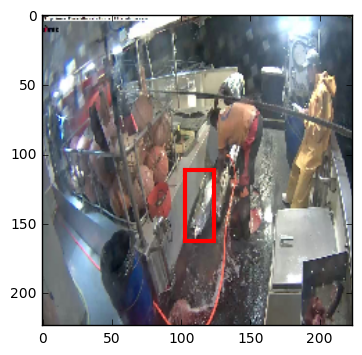
\includegraphics[width=0.5\linewidth]{box}}
\end{figure}


\subsection{Arquitectura del modelo}

Generar la caja que contiene al pez no es un problema de clasificación, porque
no tiene que distinguir entre diferentes tipos de peces, solo tiene que
identificar dónde hay uno. Esto favorecerá que la red busque características
generales de peces, en vez de características generales de cada una de las
categorías. Por otro lado, encontrar la clasificación correcta sí que requiere
buscar características específicas de cada categoría.

Al usar la misma red para ambas tareas, esta deberá encontrar un balance entre
encontrar características específicas de cada categoría y características
generales de los peces.

Para la creación de la red vamos a seguir el mismo procedimiento que en la
entrada múltiple (sección \ref{sec:multi_entry}), solo que en vez de añadir la
entrada extra en la última capa, dividiremos esta última capa en dos redes
diferentes, como se muestra en la figura \ref{multi_output_arch}.

\begin{figure}
  \caption{Arquitectura del modelo denso con salida múltiple}
\label{multi_output_arch}
  \makebox[\textwidth]{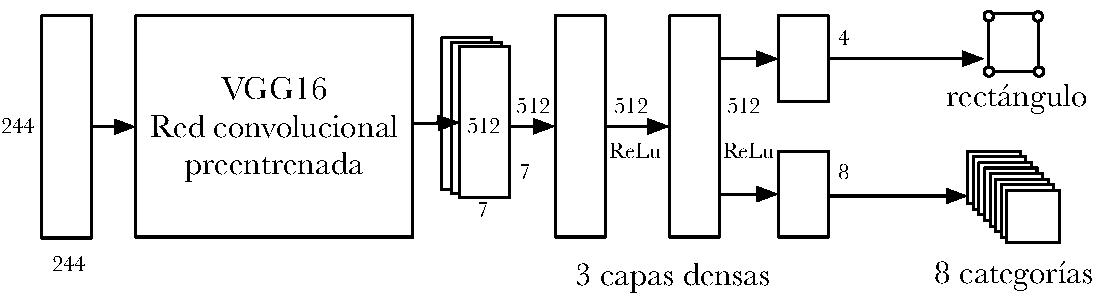
\includegraphics[width=\linewidth]{multi_output_arch}}
\end{figure}


La primera capa de salida, de localización, no posee una función de activación
ya que las cuatro salidas representa las cuatro propiedades con las que
representamos el rectángulo (x, y, altura y anchura) y es necesario que la red
indique el valor de cada una de esas cuatro propiedades.

La segunda capa es la que hemos usado hasta ahora: ocho salidas representando la
codificación \textit{onehot} de las ocho categorías.
\begin{python}
# Generar la red sin la capa de salida 
net = build_dense_layers(dropout)
# Agregar la capa de salida para la localizacion
net_bb = Dense(4, name='bb')(net)
# Agregar la capa de salida para la clasificacion
net_class = Dense(8, activation='softmax', name='class')(net)
# Generar el modelo usando la entrada + ambas capas de salida
model = Model([inp], [net_bb, net_class])
\end{python}

Al entrenar el modelo es necesario indicar de dónde sale el valor a optimizar
en cada una de las salidas. Para la nueva salida vamos a usar el error
cuadrático medio (\textit{MSE}, en inglés) entre los valores del conjunto de
datos de rectángulos y los valores generados. El \textit{MSE} consiste en la
media del cuadrado de la diferencia entre los valores esperados y los valores
de la salida. Esto penalizará mucho más los valores lejanos a la salida
esperada que los pequeños errores.

Ya que el error cuadrático será de una magnitud mayor que la pérdida logarítmica,
se pondera cada una con diferentes pesos.

\begin{python}
model.compile(
    Adam(lr=0.001),
    loss=['mse', 'categorical_crossentropy'],
    metrics=['accuracy'],
    loss_weights=[.001, 1.],  # Ponderar los errores
)
\end{python}

Ahora hay que proporcionar los ejemplos de las salidas de cada uno de los
conjuntos de datos para cada capa de salida, así como para el conjunto de
validación.

\begin{python}
model.fit(
    conv_feat,
    [trn_bbox, trn_labels],
    batch_size=batch_size,
    nb_epoch=7,
    validation_data=(conv_val_feat, [val_bbox, val_labels]),
)
\end{python}

La evaluación del modelo sobre el conjunto de test generará una evaluación para
cada capa de salida. En el cuadro \ref{eval_multi} podemos ver los valores de
cada una de las capas de salida.

\begin{table}[]
\centering
\caption{Resultados de la evaluación del modelo de salida múltiple sobre el
conjunto de test}
\label{eval_multi}
\begin{tabular}{rrr}
                       & \textbf{Pérdida} & \textbf{Precisión} \\
\textbf{Localización}  & 239.54                        & 0.8454             \\
\textbf{Clasificación} & 0.2403                        & 0.9698            
\end{tabular}
\end{table}

La precisión de la capa de clasificación, que es la que vamos a usar para la
competición, es la más alta hasta ahora. Esto puede deberse a que, como
decíamos al principio de esta sección, tiene que conseguir características para
distinguir peces así como caracterísiticas de cada categoría.

La puntuación en la tabla pública de \textit{Kaggle} para este modelo ha sido
de \textbf{0.8675}, siendo el segundo mejor modelo de los entrenados hasta ahora.

\subsection{Visualización de la localización de peces}

Como se veía en la imagen \ref{box} se puede representar la localización anotada
en el conjunto de datos de cada imagen. De la misma manera, podemos visualizar
los valores de salida de la capa de localización para ver si el modelo es capaz
de encontrar dónde se encuentra cada pez en la imagen.

En la figura \ref{predicted_boxes_1} podemos ver en rojo la localización original
y en verde la generada por el modelo. Aunque no es perfecta, captura
aproximadamente dónde se encuentra el pez. Es curioso notar que en la primera de
las dos imágenes solo está encontrando las características más visibles del pez.
La cola, que casi no es distinguible, no se incluye dentro del rectángulo
generado por el modelo.

En la segunda imagen el modelo ha sido capaz de identificar un pez, pero no el que
se le había indicado en el conjunto de entrenamiento. El pez que ha localizado
es más visible y está mejor iluminado, por lo que es más fácil de localizar. El pez
original está parcialmente tapado por la cabeza de un pescador.

\begin{figure}
  \caption{En rojo, el rectángulo correspondiente a la localización del pez en
  el conjunto de datos alternativo. En verde, el rectángulo generado por el
  modelo con salida múltiple.}
\label{predicted_boxes_1}
  \makebox[\textwidth]{
  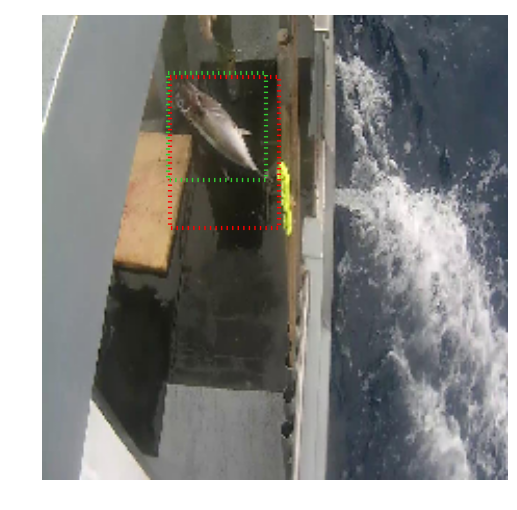
\includegraphics[width=0.5\linewidth]{predicted_boxes_1}
  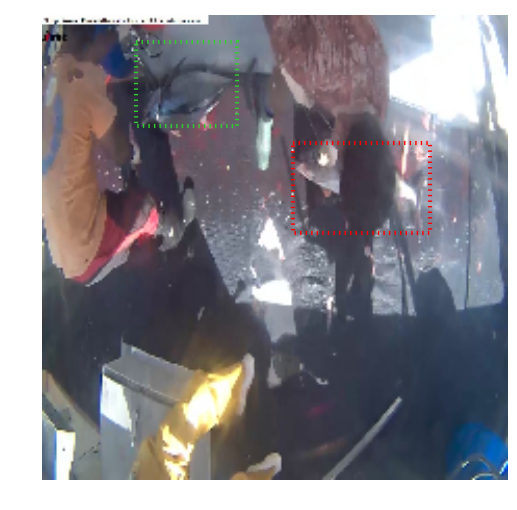
\includegraphics[width=0.5\linewidth]{predicted_boxes_2}
  }
\end{figure}


\section{Modelos \textit{ensemble}}

En competiciones de modelos predictivos es habitual que la mejor puntuación
no la obtenga un único modelo, sino un modelo construido combinando varios. Este
tipo de modelos se conocen como \textit{ensemble models} (modelos de conjunto).

Para generar estos modelos no es necesario reentrenar los modelos disponibles,
sino trabajar con las salidas de estos. Primero calculamos las predicciones de
cada modelo que queremos combinar. Luego generamos una predicción del modelo
\textit{ensemble} agregando los valores de las predicciones. Hay otros métodos
para construir modelos \textit{ensemble} más sofisticados, pero aquí se van a
considerar únicamente los más simples:

\begin{itemize}
    \item{\textbf{Votación:} La salida de cada modelo se entiende como una
            votación de a qué categoría debería pertenecer dicha entrada. La
            salida del modelo final es la elección ganadora de esa votación. Por
            ejemplo, si el modelo 1 ha elegido ALB y los modelos 2 y 3 han
        elegido YFT, la salida del modelo \textit{ensemble} será YFT.}
    \item{\textbf{Media ponderada:} En el caso de que la salida sean
            probabilidades de cada clase se puede  usar una media ponderada
            entre los valores de los modelos. La ponderación de la media permite
            dar preferencia al modelo con más confianza.
            
            En el cuadro \ref{ensemble_sample} podemos ver un ejemplo de cómo
        sería la salida de un modelo \textit{ensemble} ejemplo usando una media
    aritmética entre tres modelos diferentes.}
\end{itemize}

Debido a que los modelos presentados generan un vector de probabilidades para
cada categoría, los modelos \textit{ensemble} generados usarán la media
ponderada.

\begin{table}[]
\centering
\caption{Predicciones de diferentes modelos para una imagen, unidas en un modelo
final mediante una media aritmética}
\label{ensemble_sample}
\begin{tabular}{rllllllll}
Modelo              & ALB   & BET   & DOL   & LAG   & NoF   & OTHER & SHARK  & YFT  \\
\hline
Salida múltiple     & 0.010 & 0.052 & 0.030 & 0.001 & 0.123 & 0.079 & 0.046 & 0.875\\
Red base            & 0.020 & 0.001 & 0.030 & 0.002 & 0.123 & 0.079 & 0.046 & 0.844\\
Red convolucional   & 0.030 & 0.301 & 0.029 & 0.001 & 0.123 & 0.079 & 0.046 & 0.502\\
\hline
Ensemble            & 0.020 & 0.118 & 0.030 & 0.001 & 0.123 & 0.079 & 0.046 & 0.740
\end{tabular}
\end{table}

Usar la pérdida logarítmica como métrica hace que se castigue mucho las bajas
probabilidades en las categorías correctas. Usar la media para estos modelos
puede ayudar a evitar este comportamiento, ya que solo tendrán probabilidades
cercanas a cero aquellas categorías que sean casi cero en todos los modelos.

Un ejemplo puede verse en la categoría LAG del cuadro \ref{ensemble_sample}.
Todas los modelos predicen una baja puntuación para esa categoría, por lo que la
puntuación final también es muy baja. Sin embargo en la categoría BET existe un
modelo que le da una puntuación media, haciendo que esta se aleje de cero. En
cuanto uno de los modelos no está de acuerdo en que la puntuación sea cero, esta
se aleja.

\subsection{Resultados}

Se han presentado dos modelos diferentes usando esta técnica. Ambos modelos
están compuestos de tres modelos anteriores:

\begin{itemize}
    \item{Modelo con clasificador denso, \textit{dropout}, normalización por lotes y
        aumento de datos.}
    \item{Modelo completo convolucional}
    \item{Modelo con salida múltiple}
\end{itemize}

Estos tres modelos son los que mejores resultados obtuvieron previamente, así
que se usarán para generar dos modelos. El primero usará la media aritmética de
la salida mientras que el segundo será ponderado de la siguiente manera: 25 \%
para el clasificador denso, 25 \% para el modelo con salida múltiple y 50 \%
para el modelo completo convolucional.

Al evaluar estos modelos en \textit{Kaggle}, los resultados de la tabla pública
son los siguientes

\begin{itemize}
    \item{Media aritmética sobre los tres modelos: \textbf{0.9175}
    \item{Media ponderada favoreciendo el modelo completo convolucional: \textbf{0.8975}
\end{itemize}

Desafortunadamente las puntuaciones de \textit{ensemble}, que tradicionalmente suelen conseguir las mejores posiciones en las competiciones de \textit{Kaggle}, no han conseguido ser las mejores.

\section{Modelos finales presentados}

En los cuadros \ref{model_id} y \ref{final_scores} se presenta un resumen de
los modelos presentados, junto a sus puntuaciones.

Las reglas de la competición establecen que solo es posible puntuar dos modelos
en la tabla de puntuaciones privada y solo es posible usar un modelo para la
segunda fase.

El mejor modelo según las puntuaciones públicas de la primera fase es el que
usa un clasificador convolucional en las últimas capas, seguido del que usa una
salida múltiple para intentar clasificar los peces. Hay que recordar que estas
puntuaciones se calculan usando un subconjunto del conjunto de test, por lo que
puede cambiar cuando se publique la tabla privada.

Tradicionalmente los modelos \textit{ensemble} consiguen mejores puntuaciones
en las competiciones de \textit{Kaggle}, por lo que se ha decidido enviar un
modelo \textit{ensemble} (el tercero en mejor puntuación) y el convolucional
completo.

Al publicarse las puntuaciones privadas, vemos en el cuadro \ref{final_scores}
que el modelo convolucional consigue mejor puntuación, así que es seleccionado
como el modelo final a enviar.

La puntuación final de este modelo es de \textbf{0.907} en la tabla pública y
\textbf{1.998} en la privada, consiguiendo una posición 210 de 2293
participantes y una medalla de bronce (por clasificar dentro del mejor 10 \% de
los participantes).

\begin{table}[]
\centering
\caption{Identificadores de los modelos}
\label{model_id}
\begin{tabular}{rl}
\textbf{Id} & \textbf{Modelo}                                                       \\ \hline
vgg         & VGG16 con ajuste fino                                                 \\
v-512       & VGG16 con capas de 512 salidas                                        \\
v-norm      & VGG16 con normalización por lotes (+ 512 s, \textit{dropout})       \\
v-aug       & VGG16 con aumento de datos (+ 512 s, \textit{dropout}, norm.)       \\
v-fcn       & VGG16 con red convolucional (+ norm.)                                 \\
m-in        & VGG16 con entrada múltiple (+ 512 s, \textit{dropout}, norm, datos) \\
m-out       & VGG16 con salida múltiple (+ 512 s, \textit{dropout}, norm, datos)  \\
e-arit      & \textit{Ensemble} con media aritmética                              \\
e-pond      & \textit{Ensemble} con media aritmética ponderada                   
\end{tabular}
\end{table}

\begin{table}[]
\centering
\caption{Identificadores de los modelos}
\label{final_scores}
\begin{tabular}{r|lllll}
\textbf{Id}           & \textbf{Local}        & 1ª fase                      &                              & 2ª fase                      &                              \\ \cline{3-6} 
\multicolumn{1}{l|}{} & \multicolumn{1}{l|}{} & \multicolumn{1}{l|}{Pública} & \multicolumn{1}{l|}{Privada} & \multicolumn{1}{l|}{Pública} & \multicolumn{1}{l|}{Privada} \\ \hline
vgg                   & 2.383                 & 2.632                        & -                            & -                            & -                            \\
v-512                 & 1.272                 & 2.381                        & -                            & -                            & -                            \\
v-norm                & 0.451                 & 1.017                        & -                            & -                            & -                            \\
da-aug                & 0.312                 & 0.936                        & -                            & -                            & -                            \\
fcn                   & 0.243                 & 0.811                        & 0.770                        & 0.907                        & 1.998                        \\
m-in                  & 0.373                 & 1.047                        & -                            & -                            & -                            \\
m-out                 & 0.240                 & 0.867                        & -                            & -                            & -                            \\
e-arit                & -                     & 0.917                        & -                            & -                            & -                            \\
e-pond                & -                     & 0.897                        & 0.841                        & -                            & -                           
\end{tabular}
\end{table}
